\documentclass[a4paper,10pt]{article}
\usepackage[utf8]{inputenc}

\setlength\parindent{0pt}
\usepackage[english]{babel}
\usepackage[dvinames]{xcolor}
\usepackage[compact,small]{titlesec}
\usepackage{booktabs}
\usepackage{multirow}
\usepackage{amsfonts,amsmath,amssymb}
\usepackage{marginnote}
\usepackage[top=1.8cm, bottom=1.8cm, outer=1.8cm, inner=1.8cm, heightrounded, marginparwidth=2.5cm, marginparsep=0.5cm]{geometry}
\usepackage{enumitem}
\setlist{noitemsep,parsep=2pt}
\newcommand{\highlight}[1]{\textcolor{kuleuven}{#1}}
\usepackage{pythonhighlight}
\usepackage{cleveref}
\usepackage{graphicx}
\usepackage{algorithmic}
\usepackage{tabularx}

\newcommand{\nextyear}{\advance\year by 1 \the\year\advance\year by -1}
\newcommand{\thisyear}{\the\year}
\newcommand{\deadlineGroup}{November 27, \thisyear{} at 16:00 CET}
\newcommand{\deadlineCode}{December 18, \thisyear{} at 16:00 CET}
\newcommand{\deadlineReport}{January 4, \nextyear{} at 16:00 CET}

\newcommand{\ReplaceMe}[1]{{\color{blue}#1}}
\newcommand{\RemoveMe}[1]{{\color{purple}#1}}

\setlength{\parskip}{5pt}

%opening
\title{Artificial Neural Networks: Exercise session 1}
\author{Stijn Staring (r0620003)}

\begin{document}
\fontfamily{ppl}
\selectfont{}

\maketitle

%\section{\RemoveMe{Formal requirements}} \label{sec_this}

\section{Exercises of Section 2}
\textbf{Function approximation: comparison of various algorithms:
	Take the function $y = sin(x2) for x = 0 : 0:05 : 3$ and try to approximate it using a neural network with one hidden
	layer. Use different algorithms. How does gradient descent perform compared to other training algorithms?}\\

\textbf{Learing from training data without noise}\\
The neural network that is used in this section consists of one hidden layer with $ 50 $ hidden neurons and a single input and output neuron. The input data for training is a 1D array of $ 189  $ values. 
The results of training the neural network on training data without additive noise can be seen in Table \ref{tab:corr_with_noise}. The results are an average of $ 10 $ iterations while during each iteration the correlation coefficient between predictions and targets of a test set is calculated for a different amount of epochs. Als, a mean square value is determined after $ 1000 $ epochs based on a test set. The testset consists out of $ 3142 $ drawn points form the target function $ sin(x^2) $. $ 10 $ different random weight initializations are used which are the same $ 10 $ for all the different methods in order to make a better comparison.\\

It can be seen that the gradient descent and the gradient descent with adaptive learning rate are clearly outperformed by the other methods in function of the number of epochs. When learning on noiseless trainingdata the last three methods in the table achieve a negligible error. The Bayesian Reularization Backpropagation makes in the Matlab software also use of the ``Levenberg-Marquardt'' method which explains their similar behaviour. The ``Levenberg-Marquardt'' attains already after one epoch a better correlation coefficient between the predicted and target values of the regression than the gradient descent based methods. It can be concluded that the ``Levenberg-Marquardt'' method achieves the best result based on Table \ref{tab:corr_no_noise}.\\

It is important to note that the disadvantage of the gradient descent method in comparison with the other methods is that it has slow convergence in function of the amount of epochs but one epoch is not so calculation expensive. Using the amount of epochs as stopping criteria works therefore in the advantage of methods that converge fast in function of the number of epochs but where one epoch is expensive to calculate e.g. quasi Newton methods. Therefore, it is expected that when a time limit is used as stopping criteria, instead of the number of epochs, this will be in favour of the gradient descent based methods. \\

\begin{table}
	\centering
	\begin{tabular}{@{}l|lccr@{}} \toprule
		\textbf{Learning rule}    & $ 1 $ epoch & $ 15 $ epochs & $ 1000 $ epochs & MSE \\\midrule
		\textbf{Gradient Descent}    & $ -8.00\times10^{-3} $  & $ 1.70\times10^{-2} $  & $ 6.30\times10^{-1} $ & $ 2.86\times10^{-1} $ \\
		\textbf{GD with adaptive learning rate} & $ -8.00\times10^{-3} $  & $ 2.40\times10^{-2} $  & $ 8.86\times10^{-1} $ & $ 1.05\times10^{-1} $  \\
		\textbf{Fletcher-Reeves} & $ 1.20\times10^{-2} $  & $7.50\times10^{-1} $  & $ 9.99\times10^{-1} $ & $ 1.00\times10^{-3} $ \\
		\textbf{Polak-Ribier} & $ 1.20\times10^{-2} $  & $ 7.50\times10^{-1} $  & $ 9.99\times10^{-1} $ & $ 1.00\times10^{-3} $  \\
		\textbf{BFGS} & $ 1.10\times10^{-2} $  & $ 8.70\times10^{-1} $  & $ 1.00 $ & $ 0.0 $ \\
		\textbf{Levenberg-Marquardt} & $ 8.22\times10^{-1} $  & $ 9.95\times10^{-1} $  & $ 1.00 $ & $ 0.0 $ \\
		\textbf{Bayesian Regularization Backpropagation} & $ 8.29\times10^{-1} $  & $ 9.79\times10^{-1}$  & $ 1.00 $ & $ 0.0 $ \\ \bottomrule
	\end{tabular}
	\caption{Average correlation coefficient and MSE result over $ 10 $ iterations, making use of the predictions for the test set and learning from noiseless training data.}
	\label{tab:corr_no_noise}
\end{table}

%The performance of further methods with respect to the correlation coefficient is given in table \ref{tab:corr_no_noise} Using the ``Fletcher-Reeves'' conjugate gradient algorithm to update the weights decisevely outperforms a simple gradient descent in function of the amount of epochs. Already after $ 15 $ epochs a correlation coefficient of $ R = 0.736 $ is achieved and after $ 1000 $ epochs there is almost perfect regression with $ R = 0.99 $.\\

\textbf{Learing from training data noise}\\
Now a regression with the same neural network with one hidden layer and $ 50 $ hidden states is trained on training data with added gaussian noise. The noise has a standard deviation of $ 0.2 $ and a mean of zero. The results of the training are obtained in the same way as was done while learning from training data without noise and by making used of the same test set. The results can be seen in Table \ref{tab:corr_with_noise}.\\

All methods (except the gradient descent method) behave slightly worse when training on data with noise. The reason that the gradient descent is not affected by the noise, is because the method was also not able to do a satisfying regression on training data without noise. Therefore, it still remains not able to give satisfying results for the regressions also with noise within $ 1000 $ epochs. Because of the additive noise and no use of early stopping or a regulation term, the neural networks are vulnerable to learn less good generalizations. As will be discussed in section \ref{s:ex5} the Bayesian Regularization Backpropagation is the only one that does take a regularization term into account. This explains why this method behaves best on the noisy training data based on Table \ref{tab:corr_with_noise}.

\begin{table}
	\centering
	\begin{tabular}{@{}l|lccr@{}} \toprule
		\textbf{Learning rule}    & $ 1 $ epoch & $ 15 $ epochs & $ 1000 $ epochs & MSE \\\midrule
		\textbf{Gradient Descent}    & $ -6.00\times10^{-3} $  & $ 2.20\times10^{-2} $  & $ 7.22\times10^{-1} $ & $ 2.25\times10^{-1} $ \\
		\textbf{GD with adaptive learning rate} & $ -6.00\times10^{-3} $  & $ 3.20\times10^{-2} $  & $ 8.56\times10^{-1} $ & $ 1.27\times10^{-1} $  \\
		\textbf{Fletcher-Reeves} & $ -4.00\times10^{-3} $  & $6.84\times10^{-1} $  & $ 9.82\times10^{-1} $ & $ 1.80\times10^{-2} $ \\
		\textbf{Polak-Ribier} & $ -4.00\times10^{-3} $  & $ 6.98\times10^{-1} $  & $ 9.82\times10^{-1} $ & $ 1.80\times10^{-2} $  \\
		\textbf{BFGS} & $ -5.00\times10^{-3} $  & $ 8.72\times10^{-1} $  & $ 9.87\times10^{-1} $ & $ 2.20\times10^{-2} $ \\
		\textbf{Levenberg-Marquardt} & $ 7.71\times10^{-1} $  & $ 9.63\times10^{-1} $  & $9.53\times10^{-1} $ & $ 5.00\times10^{-2} $ \\
		\textbf{Bayesian Regularization Backpropagation} & $ 8.17\times10^{-1} $  & $ 9.55\times10^{-1}$  & $ 9.82\times10^{-1} $ & $ 1.70\times10^{-2} $ \\ \bottomrule
	\end{tabular}
	\caption{Average correlation coefficient and MSE result over $ 10 $ iterations, making use of the predictions for the test set and learning from training data with gaussian noise.}
	\label{tab:corr_with_noise}
\end{table}

\textbf{In this problem, the objective is to approximate a non-linear function using a feedforward artificial neural network.} \textbf{Define your datasets: your dataset consists now of X1;X2 and Tnew. Draw 3 (independent) samples of $ 1 000 $ 	points each. Use them as the training set, validation set, and test set, respectively. Motivate the choice of the 	datasets. Plot the surface of your training set using the Matlab function scatteredInterpolant,plot3 and mesh.}\\

Three datasets are developed respectively for training, validation and testing. The training dataset is usually the largest and has as purpose to learn the weights of the network. This is done by making use of the backpropagation algorithm to calculate the gradient and  the learning rules as discussed in the previous discussed tables. The purpose of the validation set is to find the best suitable hyper parameters and tune design decisions of the neural network e.g. amount of neurons, amount of layers. A test set is used to determine the performance of the network on unseen data. Figure \ref{fig:surface} shows the surface that is the learning target of the training dataset. 

\begin{figure}[h!]
	\centering
	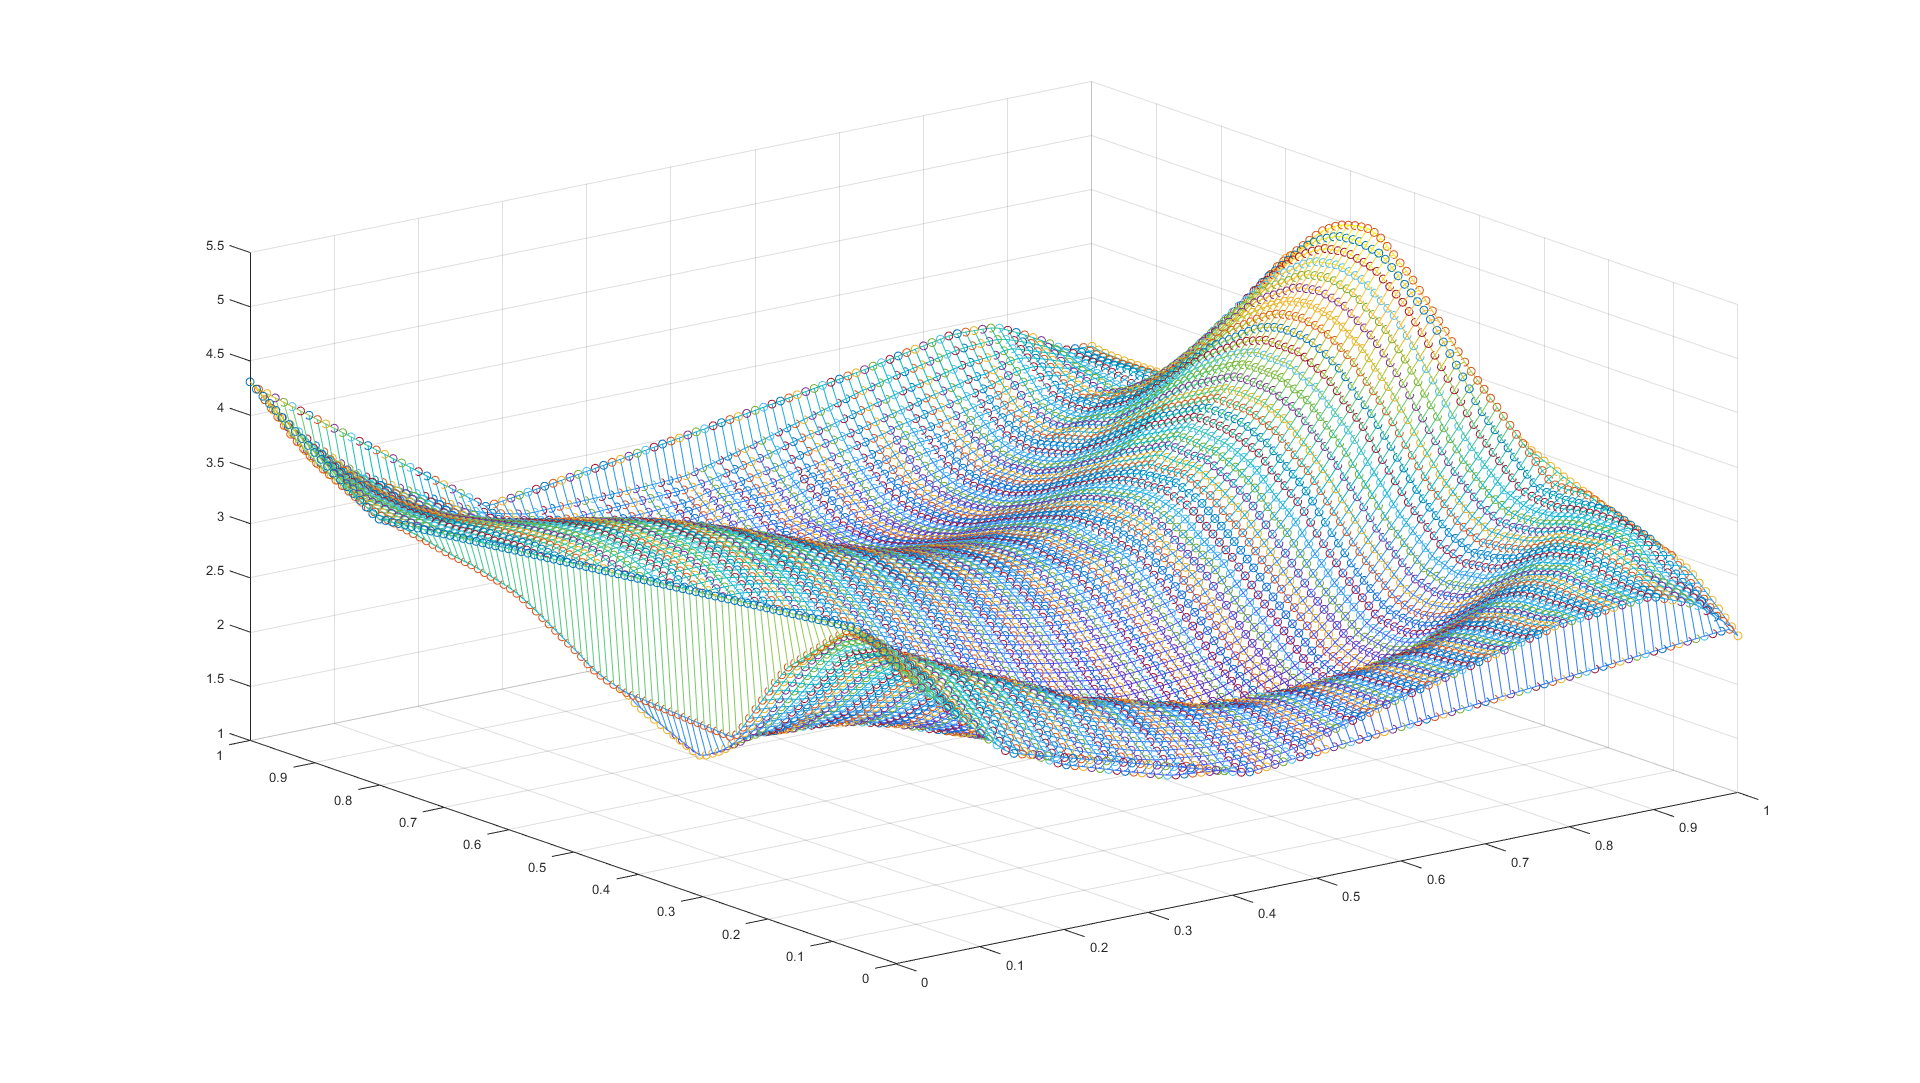
\includegraphics[width=0.4\textwidth]{surface.png}
	\caption{The visualization of the target surface of the training set.}
	\label{fig:surface}
\end{figure}


\textbf{Build and train your feedforward Neural Network: use the training and validation sets. Build the ANN with 2	inputs and 1 output. Select a suitable model for the problem (number of hidden layers, number of neurons in each hidden layer). Select the learning algorithm and the transfer function that may work best for this problem.
	Motivate your decisions. When you try different networks, clearly say at the end which one you would select as
	the best for this problem and why.}\\

The feedforward neural network is build by using the Deep Learning Toolbox in Matlab. Table \ref{tab:design} shows an overview of design decisions that have been tried. Each combination is run $ 10 $ times from which the average mean square error is calculated on the validation set. In order to deal with overfitting the validation set is also used to perform early stopping. This means that during training the error on the validation set may only $ 10 $ times increase directly after each other. If this amount is exceeded the learning is stopped. Early stopping is the default measure to deal with overfitting in the Matlab Deep Learning toolbox. Additionally, to avoid overfitting a regulation term is added in the objective function during training. This regulation term is the L2 norm of the weights and a regulation parameter is used to determine the importance of the regulation term in comparison with the training error on the targets.\\

 The training is stopped when the max amount of $ 500 $ iterations is reached, the training error becomes smaller then $ 10^{-3} $ or when the learning takes longer then $ 1 $ minute. The activation functions that are used are the default ones of the Matlab toolbox. For a hidden layer and the output layer these are respectively the ``tansig'' and ``purelin'' functions.
It was found after simulations that the smallest average MSE is obtained when the neural network has a regulation parameter of zero, two hidden layers of each five neurons and uses the gradient descent learning rule. \\


\begin{table}
	\centering
	\begin{tabular}{@{}lr@{}} \toprule
		\textbf{Design Variable}    & Domain \\\midrule
		Regulation parameter & $ 0 $ or $ 0.2 $  \\ 
		Amount of hidden layers & $ 1 $ or $ 2 $  \\
		Amount of neurons per layer & $ 5:5:100 $  \\
		Learning rule & all from Table \ref{tab:corr_no_noise}\\
		Training time per training session & $ 120 s $\\
		Max amount of epochs & $ 1000 $\\
		Max amount of sequential increases of the validation error & $ 10 $\\
		Goal of training error & $ 10^{-3} $\\
		Amount of iterations of average MSE & $ 10 $\\\bottomrule
	\end{tabular}
	\caption{The different design variable and their corresponding domain that were varied.}
	\label{tab:design}
\end{table}


\textbf{Performance Assessment: evaluate the performance of your selected network on the test set. Plot the surface of
	the test set and the approximation given by the network. Plot the error level curves. Compute the Mean Squared
	Error on the test set. Comment on the results and compare with the training performance. What else could you
	do to improve the performance of your network?}\\

Now the performance of the learned neural network is assessed. The network with the best performance on the validation set is trained for $ 5 $ minutes.
Figure \ref{fig:After_simulation_of_5min_per} shows the distribution of the errors between the target values and the obtained predictions. A correlation coefficient of $ R = 98.3 $ is reached between target and prediction values on the test set which means there is a linear correlation. 
Figure \ref{fig:errorSurface} shows the error between the targets and the predictions of the test set. The plane is calculated by subtracting the learned plane from the target plane. It can be seen that especially in the middle the neural network performed a better regression than on the sides. \\
Things that could be done to improve the network are a more extensive parameter search e.g. also looking in networks with different amount of neurons in the hidden layers and looking at the possibility to combine different learned networks. 

%It can be seen that at the end the error on the test set is smaller than the error on the training set. This is possible however, this is normally not the case because the test set is data that is never seen by the network before. The MSE error on respectively the training and the test set is $ 1.29 \times 10^{-2} $ and $ 1.12 \times 10^{-2} $. \\ 


% and Figure \ref{After_similation_of_5min} shows the correlation between the target and prediction values of the test set. It can be seen that there is a correlation coefficient of $ R = 98.3 $ which means there is almost a perfect correlation.\\ 


%Figure \ref{fig:After_simulation_of_5min} gives the evolution of the error on the training, validation and test set in function of the number of epochs during training.
%Figure \ref{fig:learnedSet} shows in red the target surface and in blue the learned surface. Figure \ref{fig:errorSurface} shows the difference between the two planes by subtracting the learned plane from the target plane. It can be seen that especially in the middle the neural network learned better predictions than on the sides. 




%\begin{figure}[h!]
%	\centering
%	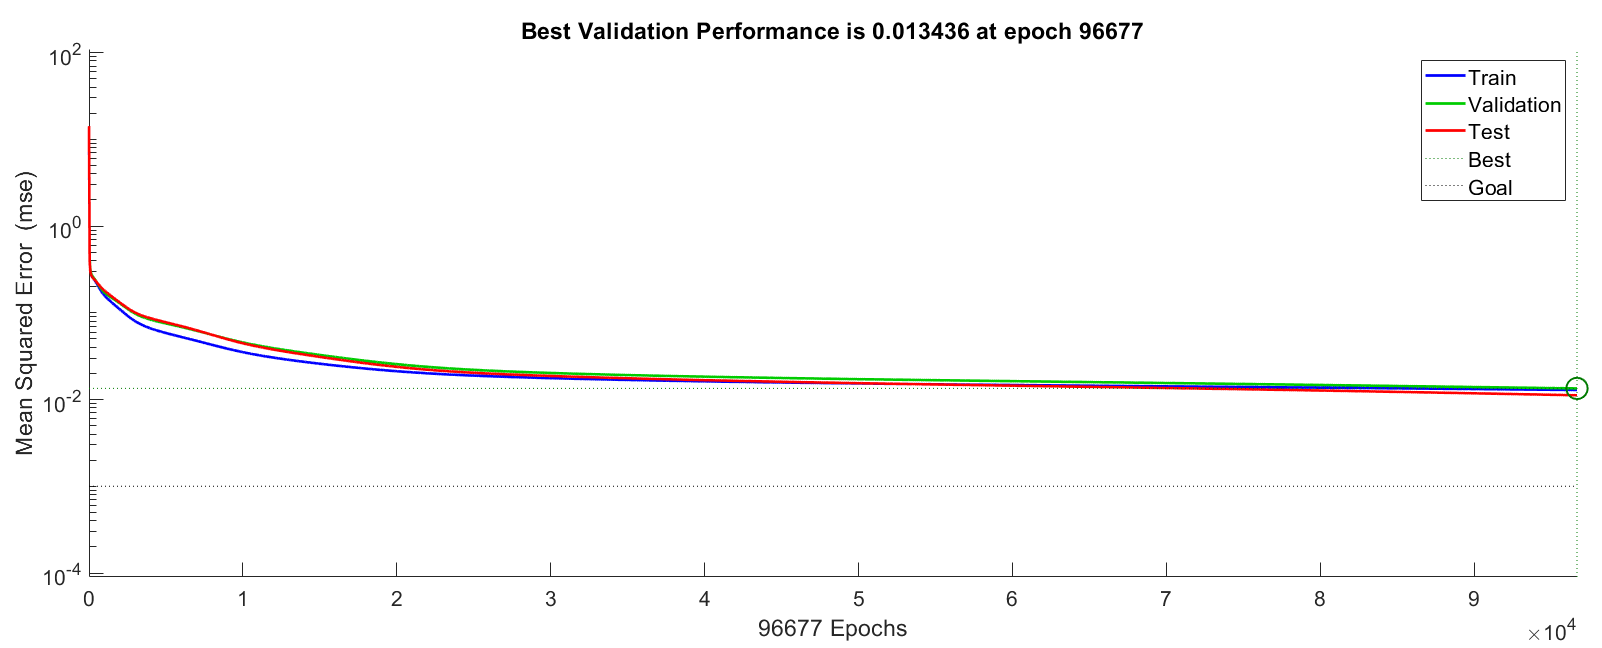
\includegraphics[width=1\textwidth]{After_simulation_of_5min.png}
%	\caption{The decrease of training, validation and test set error in function of the number of epochs.}
%	\label{fig:After_simulation_of_5min}
%\end{figure}

\begin{figure}[h!]
	\centering
	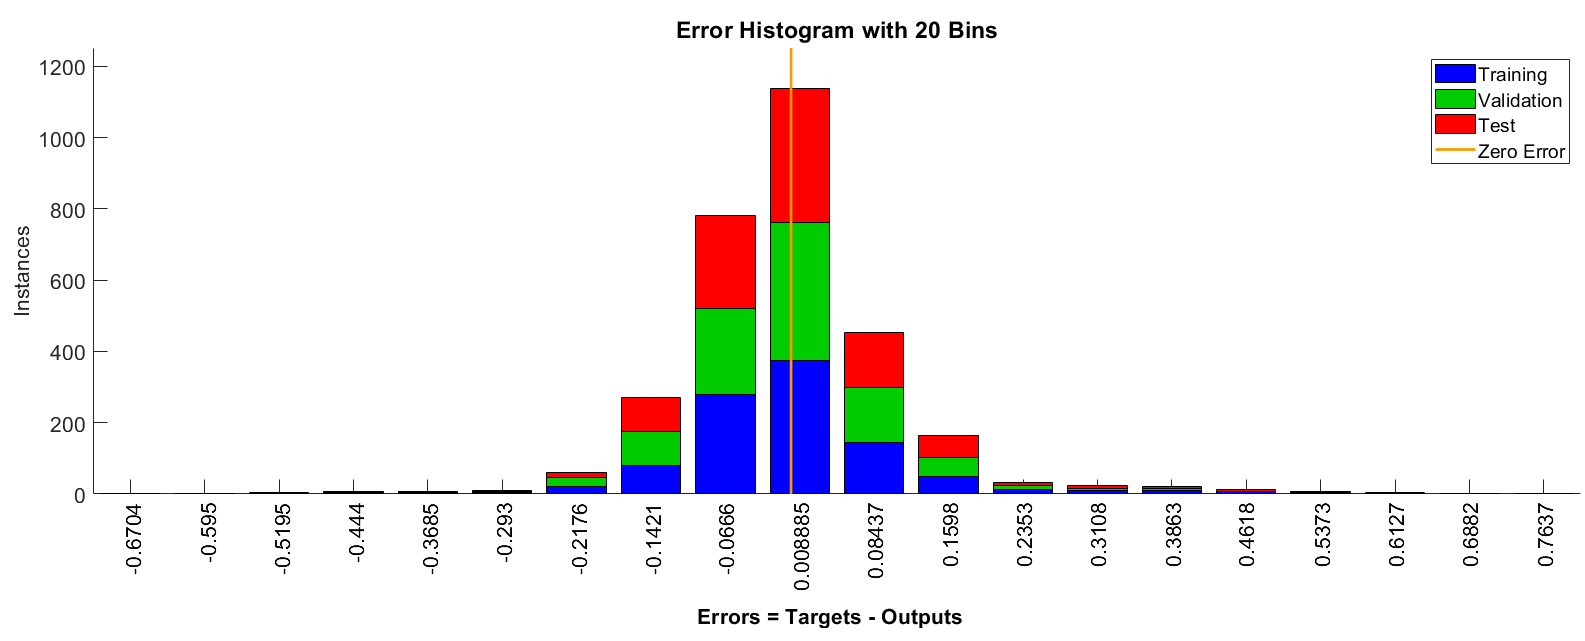
\includegraphics[width=1\textwidth]{After_simulation_of_5min_per.png}
	\caption{The distribution of the errors of the training, validation and test sets.}
	\label{fig:After_simulation_of_5min_per}
\end{figure}

%\begin{figure}[h!]
%	\centering
%	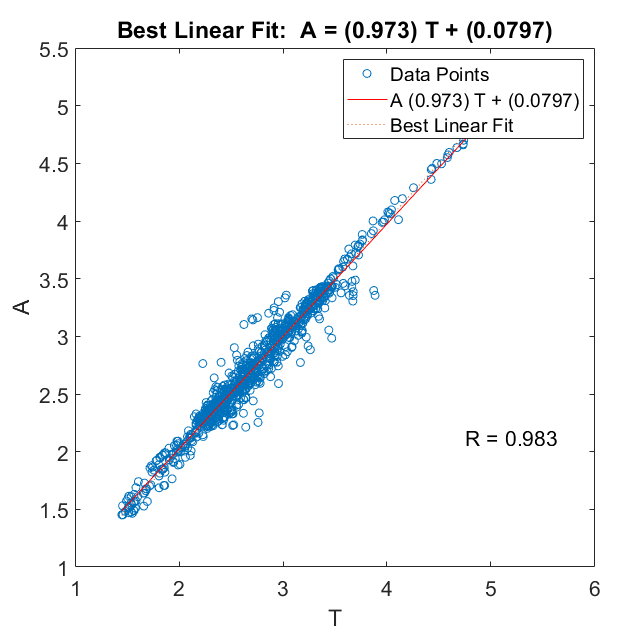
\includegraphics[width=0.5\textwidth]{After_similation_of_5min.png}
%	\caption{The correlation between the target and predicted values of the test set.}
%	\label{fig:After_similation_of_5min}
%\end{figure}


%\begin{figure}[h!]
%	\centering
%	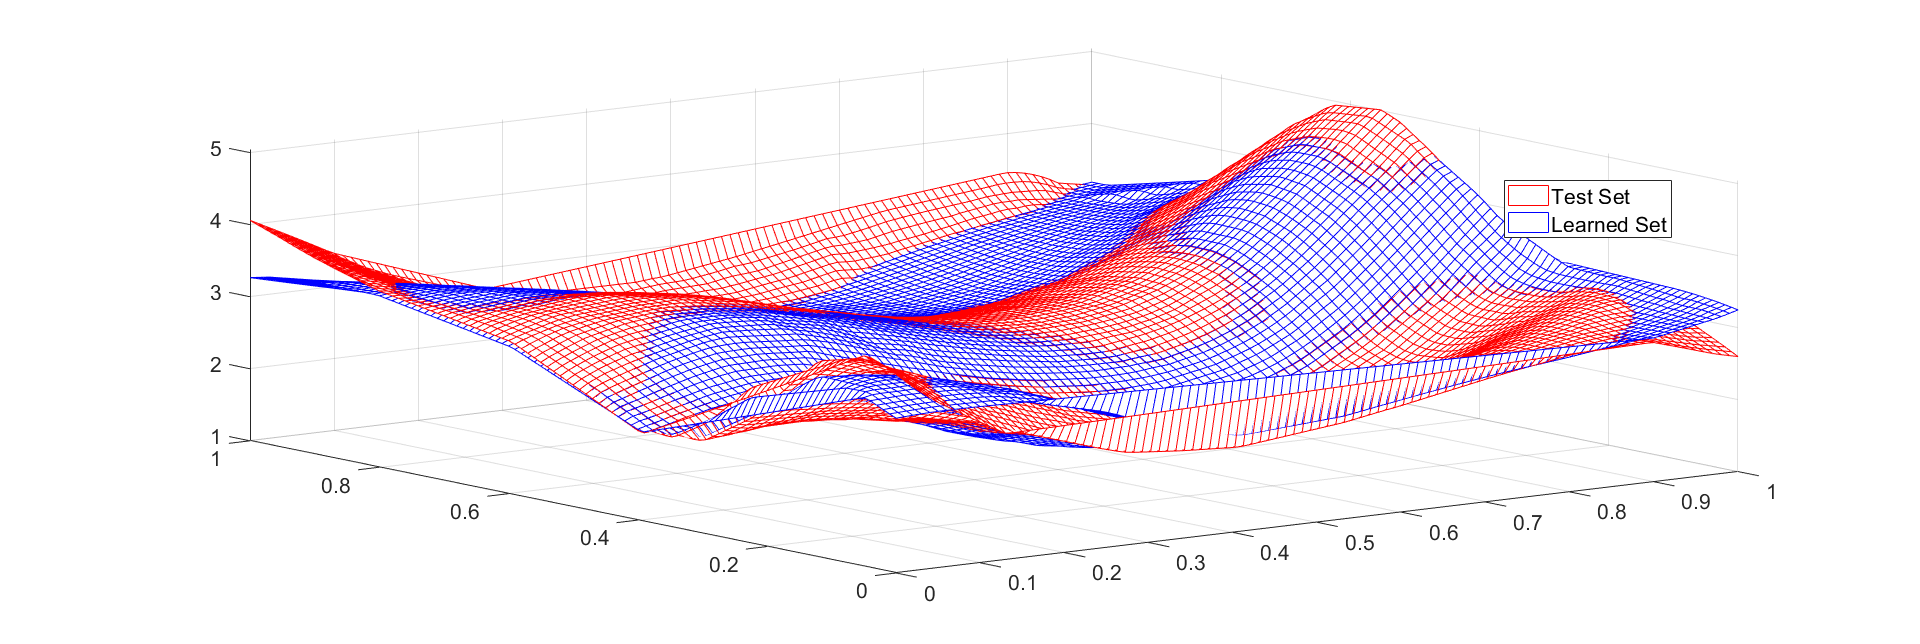
\includegraphics[width=0.8\textwidth]{learnedSet.png}
%	\caption{In red the target plane and in blue the learned plane are shown.}
%	\label{fig:learnedSet}
%\end{figure}

\begin{figure}[h!]
	\centering
	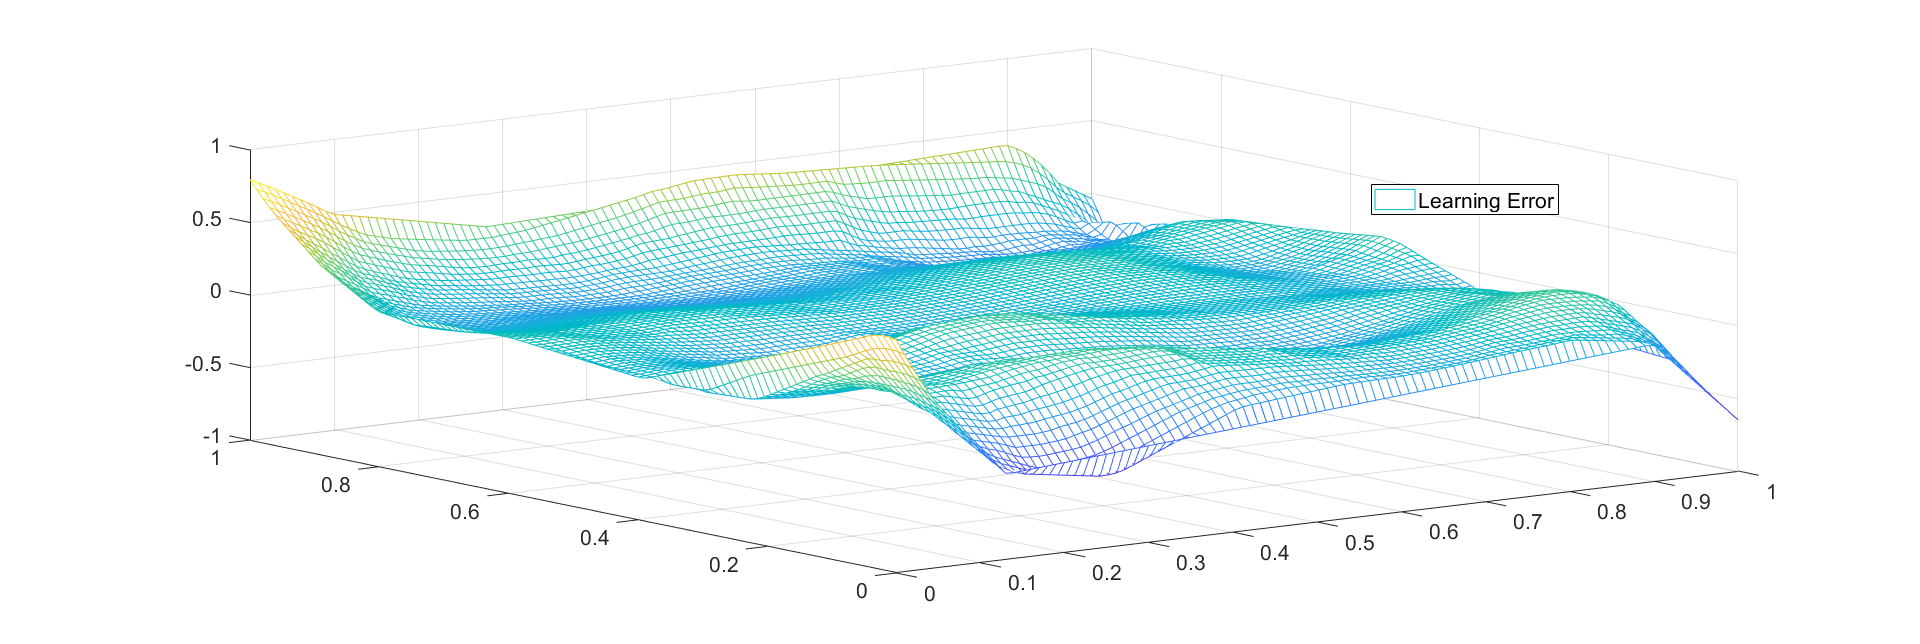
\includegraphics[width=0.6\textwidth]{errorSurface.png}
	\caption{The error plane that shows the difference between the target and the learned plane.}
	\label{fig:errorSurface}
\end{figure}


%\begin{figure}[h!]
%	\centering
%	\includegraphics[width=1.0\textwidth]{RNN.png}
%	\caption{Figure of the logical flow of a vanilla RNN with a hidden state (source \cite{Czum2020}).}
%	\label{fig:RNN}
%\end{figure}

%\begin{table}
%  \centering
%  \begin{tabular}{@{}llr@{}} \toprule
%    \multicolumn{2}{c}{Item} \\ \cmidrule(r){1-2}
%    Animal    & Description & Price (\$)\\ \midrule
%    Gnat      & per gram    & 13.65 \\
%              & each        & 0.01 \\
%    Gnu       & stuffed     & 92.50 \\
%    Emu       & stuffed     & 33.33 \\
%    Armadillo & frozen      & 8.99 \\ \bottomrule
%  \end{tabular}
%  \caption{A table with the correct layout.}
%  \label{tab:ok}
%\end{table}
\newpage
\section{Exercises of Section 5}\label{s:ex5}
\textbf{Use trainbr to analyse the first two datasets of section 2 (the function y = sin(x2) and the noisy version) and compare it with the other training algorithms investigated there. Compare the test errors. Consider overparametrized networks (many neurons): do you see any improvement with trainbr?}\\

The Bayesian regularization backpropagation method behaved similar as the ``Levenberg-Marquardt'' learning rule and very rapidly obtained a good correlation coefficient in function of the amount of epochs in Tables \ref{tab:corr_no_noise} and \ref{tab:corr_with_noise}. However, the method distinguishes itself by taking a combination of the squared errors and weights into account from which the hyper parameters, that indicates the importance of both terms, are automatically obtained. Because now a regularization term is used it is expected that the Bayesian regularization backpropagation method can better deal with noisy data.This could also be seen in Table \ref{tab:corr_with_noise} where the bayesian regularization backpropagation method performs the best on noisy training data. Tabel \ref{tab:over_para} gives the performance on an overparameterized network consisting of $ 1 $ hidden layer with $ 100 $ neurons and learning from noisy training data. The smallest MSE error is found using the Bayesian regularization backpropagation method. It can be noted that the regulation term was able to mittigate the influence of overparameterization by reducing the effictive number of parameters. This explains the difference in MSE error between the bayesian regularization backpropagation and ``Levenberg-Marquardt'' method found in Table \ref{tab:over_para}.\\
 All the other methods perform slightly worse on the overparameterized network. The reason for this is the absence of a regularization term.



%attains a good correlation coefficient after one epoch as can be seen in Tables \ref{tab:corr_no_noise} and \ref{tab:corr_with_noise}. This is similar as the ``Levenberg-Marquardt'' learning rule. However, the method distinguishes itself by taking a combination of the squared errors and weights into account from which the hyper parameters that determine the importance of both terms, are automatically obtained.

% Because now a regularization term is used it is expected that the Bayesian regularization backpropagation method can better deal with noisy data.This could also be seen in Table \ref{tab:corr_with_noise} where the bayesian regularization backpropagation method performs the best on noisy training data. while at first it had similar performance on training data without noise. \\ Tabel \ref{tab:over_para} gives the performance on an overparameterized network consisting of $ 1 $ hidden layer with $ 100 $ neurons and learning from noisy training data.  The effect of over parametrization causes a bigger error with the test set in  Table \ref{tab:over_para} then was obtained in Table \ref{tab:corr_with_noise}. This can be seen on all methods except for the gradient descent. The calculation of the MSE is made by considering $ 3142 $ samples of the sinus function without noise.\\

\begin{table}
	\centering
	\begin{tabular}{@{}l|lccr@{}} \toprule
		\textbf{Learning rule}    & $ 1 $ epoch & $ 15 $ epochs & $ 1000 $ epochs & MSE \\\midrule
		\textbf{Gradient Descent}    & $ 2.60\times10^{-2} $  & $ 8.00\times10^{-2} $  & $ 7.80\times10^{-1} $ & $ 2.18\times10^{-1} $ \\
		\textbf{GD with adaptive learning rate} & $ 2.60\times10^{-2} $  & $ 7.20\times10^{-2} $  & $ 7.90\times10^{-1} $ & $ 2.08\times10^{-1} $  \\
		\textbf{Fletcher-Reeves} & $ -5.00\times10^{-3} $  & $6.28\times10^{-1} $  & $ 9.72\times10^{-1} $ & $ 3.00\times10^{-2} $ \\
		\textbf{Polak-Ribier} & $ -5.00\times10^{-3} $  & $ 5.89\times10^{-1} $  & $ 9.73\times10^{-1} $ & $ 2.90\times10^{-2} $  \\
		\textbf{BFGS} & $ 2.60\times10^{-2} $  & $ 8.85\times10^{-1} $  & $ 9.39\times10^{-1} $ & $ 6.90\times10^{-2} $ \\
		\textbf{Levenberg-Marquardt} & $ 9.51\times10^{-1} $  & $ 9.70\times10^{-1} $  & $9.14\times10^{-1} $ & $ 1.12\times10^{-1} $ \\
		\textbf{Bayesian Regularization Backpropagation} & $ 9.43\times10^{-1} $  & $ 9.69\times10^{-1}$  & $ 9.58\times10^{-1} $ & $ 4.60\times10^{-2} $ \\ \bottomrule
	\end{tabular}
	\caption{Average correlation coefficient and MSE result over $ 10 $ iterations, making use of the predictions for the test set and learning from training data with gaussian noise. A NN is used with a hidden layer of $ 100 $ neurons.}
	\label{tab:over_para}
\end{table}




\bibliographystyle{abbrv}
%\bibliography{ANN1}

\end{document}
